\section{Decoherence-Free Algebraic Validation}

A persistent barrier in the development of topological quantum computers is the extreme fragility of the physical systems (e.g., fractional quantum Hall devices) required to host non-abelian anyons. Environmental interactions induce decoherence, necessitating massive physical overheads for active error correction (e.g., surface codes).

The primary advantage of the UOR Atlas lies in decoupling the mathematical validation of TQC from the physical limitations of quantum hardware. Because the computational manifold is synthesized algebraically on deterministic classical hardware, the system serves as an idealized, formal emulation environment for verifying topological properties. We emphasize that this does not imply a physical realization of a quantum computer; rather, it is a formal compiler and theorem-proving structure designed to algebraically assert the logical integrity of topological algorithms.

Furthermore, this framework delivers a structural advantage for algorithmic verification. Conventional matrix-vector simulations suffer from exponential resource demands when entangled states grow, attempting to numerically integrate continuous probability fields. By evaluating topological invariants dynamically via the non-pointed $S4$ modal logic framework, the UOR Atlas manipulates the discrete topological permutation orbit directly~\cite{boixo2018}. The computational complexity of evaluating whether two braid words collapse into the identical topological $\kappa$-form scales polynomially, governed by the combinatorial bounds of the 24 symmetry classes. This grants the academic community the ability to design, compile, and formally verify the abstract topological pathways of algorithms without attempting the classically intractable $\#P$-hard task of extracting scalar probability amplitudes.

\begin{figure}[h]
\centering
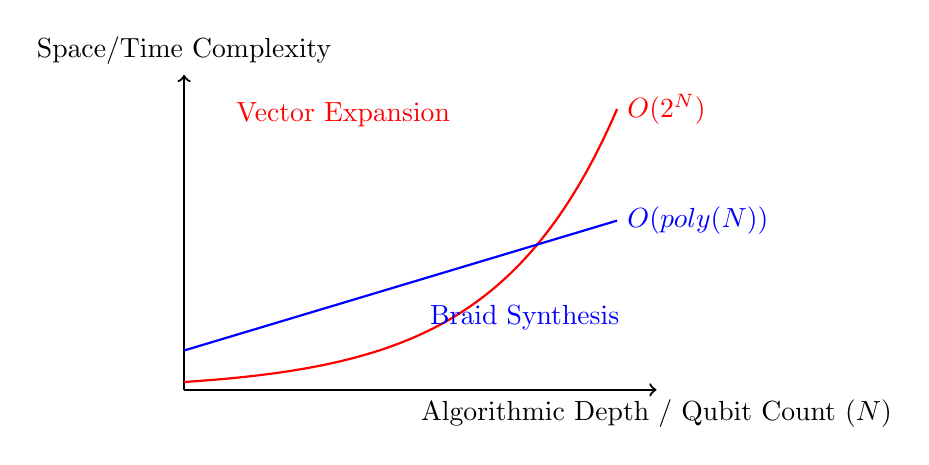
\begin{tikzpicture}
    % Axes
    \draw[thick,->] (0,0) -- (6,0) node[anchor=north] {Algorithmic Depth / Qubit Count ($N$)};
    \draw[thick,->] (0,0) -- (0,4) node[anchor=south] {Space/Time Complexity};
    
    % Exponential curve (Standard simulation)
    \draw[thick, red, domain=0:5.5, samples=100] plot (\x, {0.1*exp(0.65*\x)}) node[anchor=west] {$O(2^N)$};
    
    % Polynomial curve (Topological Compilation)
    \draw[thick, blue, domain=0:5.5, samples=100] plot (\x, {0.3*\x + 0.5}) node[anchor=west] {$O(\text{poly}(N))$};
    
    % Labels
    \node[anchor=east, text=red] at (3.5, 3.5) {Vector Expansion};
    \node[anchor=north west, text=blue] at (3, 1.2) {Braid Synthesis};
\end{tikzpicture}
\caption{Complexity comparison. Traditional quantum simulations require $O(2^N)$ classical resources to track the full state vector. The UOR Atlas restricts execution to the topological permutation space, synthesizing algorithms via bounded combinatorial braids in polynomial time.}
\label{fig:complexity}
\end{figure}
